% RAMP-VO notes final LaTeX source
\documentclass[11pt]{article}

\usepackage[a4paper,margin=1in]{geometry}
\usepackage{amsmath,amssymb,mathtools,bm}
\usepackage{graphicx}
\usepackage{tikz}
\usetikzlibrary{arrows.meta,positioning,calc,fit}
\usepackage[hidelinks]{hyperref}
\usepackage{algorithm}
\usepackage[noend]{algpseudocode}
\providecommand{\theHalgorithm}{\arabic{algorithm}}

\newcommand{\R}{\mathbb{R}}
\newcommand{\norm}[1]{\left\lVert #1 \right\rVert}
\newcommand{\T}{^{\top}}
\newcommand{\concat}{\mathbin{\|\!\|}}
\newcommand{\patch}[1]{\mathbf{P}^{#1}}
\newcommand{\projpatch}[1]{\mathbf{P}'^{#1}}
\newcommand{\state}{\boldsymbol{\Sigma}}
\newcommand{\given}{\,|\,}

\title{RAMP-VO Notes}
\author{Sebastiano Mengozzi}
\date{March 2026}

\begin{document}
\maketitle

\section{Goal and optimization variables}

RAMP-VO is a learned visual odometry system that fuses standard images and event stacks in an asynchronous way.
Its backend is inherited from DPVO: the algorithm estimates a sliding window of camera poses together with patch depths by minimizing a patch reprojection error.
For an active set of frames and patches, the optimization variables are
\begin{equation}
\mathbf{X} = \left\{ \mathbf{T}_i, d_j^l \right\},
\end{equation}
where
\begin{itemize}
    \item \(\mathbf{T}_i \in \mathrm{SE}(3)\): camera pose at time index \(i\), mapping world coordinates into camera-\(i\) coordinates,
    \item \(d_j^l \in \R\): depth associated with patch \(l\) extracted at source frame \(j\).
\end{itemize}
The backend minimizes
\begin{equation}
\label{eq:main_ba}
J(\mathbf{X}) = \sum_{(l,i)\in \mathcal{E}} \norm{\left[\hat{\mathbf{P}}_{ji}^{\prime l} + \Delta_{li}\right] - \hat{\omega}(\mathbf{T}_i,\mathbf{T}_j,\mathbf{P}_j^l)}_{\sigma_{li}}^2,
\end{equation}
where we use the shorthand
\begin{equation}
\norm{\mathbf{r}}_{\sigma_{li}}^2 := \mathbf{r}\T \sigma_{li}\mathbf{r},
\end{equation}
for a generic residual vector \(\mathbf{r}\in\R^2\) associated with edge \((l,i)\),
and define
\begin{equation}
\mathbf{P}_{ji}^{\prime l} = \omega(\mathbf{T}_i,\mathbf{T}_j,\mathbf{P}_j^l)\in\R^{4\times p^2},
\qquad
\hat{\mathbf{P}}_{ji}^{\prime l} = \hat{\omega}(\mathbf{T}_i,\mathbf{T}_j,\mathbf{P}_j^l)\in\R^{2},
\end{equation}
Here \(\mathbf{P}_j^l\in\R^{4\times p^2}\) denotes patch \(l\) extracted from source frame \(j\). The operator \(\omega(\mathbf{T}_i,\mathbf{T}_j,\mathbf{P}_j^l)\) transforms and projects all patch pixels into frame \(i\), while \(\hat{\omega}(\mathbf{T}_i,\mathbf{T}_j,\mathbf{P}_j^l)\) applies the same geometric operations and then extracts only the patch center. So the hat means: same reprojection as \(\omega\), plus center extraction.
Equivalently, without the weighted-norm shorthand,
\begin{equation}
J(\mathbf{X}) =
\sum_{(l,i)\in \mathcal{E}}
\left(
\left[\hat{\mathbf{P}}_{ji}^{\prime l} + \Delta_{li}\right] - \hat{\omega}(\mathbf{T}_i,\mathbf{T}_j,\mathbf{P}_j^l)
\right)\T
\sigma_{li}
\left(
\left[\hat{\mathbf{P}}_{ji}^{\prime l} + \Delta_{li}\right] - \hat{\omega}(\mathbf{T}_i,\mathbf{T}_j,\mathbf{P}_j^l)
\right).
\end{equation}
Using the explicit reprojection map introduced later in Section~5, the same cost can be written even more explicitly as
\begin{equation}
J(\mathbf{X}) =
\sum_{(l,i)\in \mathcal{E}}
\left(
\left[\hat{\mathbf{P}}_{ji}^{\prime l} + \Delta_{li}\right] -
\operatorname{center}\!\left(\bar{\mathbf{K}}\,\mathbf{T}_i\mathbf{T}_j^{-1}\bar{\mathbf{K}}^{-1}\,\mathbf{P}_j^l\right)
\right)\T
\sigma_{li}
\left(
\left[\hat{\mathbf{P}}_{ji}^{\prime l} + \Delta_{li}\right] -
\operatorname{center}\!\left(\bar{\mathbf{K}}\,\mathbf{T}_i\mathbf{T}_j^{-1}\bar{\mathbf{K}}^{-1}\,\mathbf{P}_j^l\right)
\right),
\end{equation}
Here \(\operatorname{center}(\cdot)\) means extraction of the patch center, so it is the same operation denoted elsewhere by the hat. Also, \(\mathcal{E}\) is the active patch--frame graph, and for each edge \((l,i)\in\mathcal{E}\), the DPVO backend predicts a learned 2D correction \(\Delta_{li}\in\R^2\) and a weight matrix \(\sigma_{li}\in\R^{2\times 2}\).
Thus RAMP-VO still solves a geometric alignment problem, but the correspondence updates \((\Delta_{li},\sigma_{li})\) are predicted by a learned asynchronous encoder and a learned update operator from the DPVO backend.

\section{Comparison with the VIO cost}

The explicit matrix form of the RAMP-VO backend cost is
\begin{equation}
J(\mathbf{X}) =
\sum_{(l,i)\in \mathcal{E}}
\left(
\left[\hat{\mathbf{P}}_{ji}^{\prime l} + \Delta_{li}\right] -
\operatorname{center}\!\left(\bar{\mathbf{K}}\,\mathbf{T}_i\mathbf{T}_j^{-1}\bar{\mathbf{K}}^{-1}\,\mathbf{P}_j^l\right)
\right)\T
\sigma_{li}
\left(
\left[\hat{\mathbf{P}}_{ji}^{\prime l} + \Delta_{li}\right] -
\operatorname{center}\!\left(\bar{\mathbf{K}}\,\mathbf{T}_i\mathbf{T}_j^{-1}\bar{\mathbf{K}}^{-1}\,\mathbf{P}_j^l\right)
\right).
\end{equation}
Using the notation of the VIO note, the weighted least-squares cost is


\begin{align}
J_{\mathrm{VIO}}(\mathbf{X}) &=
J_{\mathrm{VIO}}(\mathbf{r}_{\mathrm{prior}},\mathbf{r}_{\mathrm{imu}})
+
\sum_{(i,\ell)\in \mathcal{C}}
\left(
\mathbf{u}_{i\ell} -
\operatorname{pix}\!\left(
\mathbf{K}\frac{1}{(\mathbf{P}_{\ell}^{C_i})_z}\mathbf{P}_{\ell}^{C_i}
\right)
\right)\T
\Sigma_{i\ell}^{-1}
\left(
\mathbf{u}_{i\ell} -
\operatorname{pix}\!\left(
\mathbf{K}\frac{1}{(\mathbf{P}_{\ell}^{C_i})_z}\mathbf{P}_{\ell}^{C_i}
\right)
\right),
\end{align}
with 
\[
\mathbf{P}_{\ell}^{C_i}
=
\mathbf{R}_{CB}\!\left(\mathbf{R}_i\T(\mathbf{P}_\ell^W-\mathbf{p}_i)-\mathbf{p}_{BC}^B\right).
\]
Structurally, both are weighted sums of quadratic residual terms. The difference is that RAMP-VO uses only patch-reprojection factors over poses and patch depths, with learned corrections \(\Delta_{li}\) and learned weights \(\sigma_{li}\), while VIO combines three heterogeneous factor types: a prior term, IMU factors, and camera reprojection factors. In short, RAMP-VO has one geometrically uniform factor family enriched by neural predictions, whereas VIO merges multiple sensor-model residual families into the same least-squares objective.


\section{Asynchronous input stream}

The paper uses the word \emph{frame} for both ordinary images and event stacks.
The input is a temporally ordered asynchronous stream
\begin{equation}
\left\{ \mathbf{I}_{k_j}(t_j) \right\}_{j=1}^{T},
\end{equation}
where
\begin{itemize}
    \item \(k_j \in \{\mathrm{e},\mathrm{i}\}\) indicates whether the sample at time \(t_j\) comes from the event sensor or the image sensor,
    \item \(\mathbf{I}_{\mathrm{e}}(t_j) \in \R^{5\times H\times W}\) is an event stack,
    \item \(\mathbf{I}_{\mathrm{i}}(t_j) \in \R^{C\times H\times W}\) is an image.
\end{itemize}
The key modeling choice is that these inputs are \emph{not} forced onto one common synchronous rate.
Instead, every time a new image or event stack arrives, the internal representation is updated.
This is the main difference from a naive ``concatenate images and events'' pipeline.

\section{High-level decomposition}

For each incoming element of the asynchronous stream, RAMP-VO performs four conceptual steps:
\begin{enumerate}
    \item encode the new image/event input with the RAMP encoder to produce matching and context features,
    \item extract patches in informative regions,
    \item connect those patches to nearby frames and estimate projection corrections,
    \item run differentiable bundle adjustment to update poses and patch depths.
\end{enumerate}
Pose forecasting is then used to initialize the next pose estimate more accurately than a simple constant-velocity extrapolation.

\section{Patch representation}

Like DPVO, RAMP-VO does not optimize sparse keypoints as single pixels.
It optimizes small image patches.
For patch \(l\) extracted from source frame \(j\), the dimensionally consistent interpretation is
\begin{equation}
\mathbf{P}_j^l =
\begin{bmatrix}
\mathbf{x} \\
\mathbf{y} \\
\mathbf{1} \\
\mathbf{d}
\end{bmatrix}
\in \R^{4\times p^2},
\qquad
\mathbf{x},\mathbf{y},\mathbf{1},\mathbf{d}\in\R^{1\times p^2}.
\end{equation}
Here:
\begin{itemize}
    \item \(\mathbf{x},\mathbf{y}\) store the pixel coordinates of all \(p^2\) pixels in the patch,
    \item \(\mathbf{1}\) is a row of ones used for homogeneous coordinates,
    \item \(\mathbf{d}\) stores the depth values, taken constant within the patch in the implementation described by the paper.
\end{itemize}
So each column of \(\mathbf{P}_j^l\) corresponds to one pixel of the patch written in augmented coordinates. The paper writes this object in a compact transposed form, but taken literally that notation is ambiguous; the reprojection formula only works dimension-wise when \(\mathbf{P}_j^l\) is interpreted as a \(4\times p^2\) matrix.

The patch centers are chosen from regions with high event density:
\begin{itemize}
    \item count events per pixel to build a density map,
    \item apply non-maximum suppression over an \(11\times 11\) neighborhood,
    \item keep the \(N\) strongest surviving locations.
\end{itemize}
This is a practical design choice: if patch centers were sampled without considering event activity, many would fall in regions where events provide little or no tracking information.

\section{Patch reprojection graph}

Each source patch is connected to nearby frames within a temporal index radius \(r\), meaning that
\begin{equation}
|i-j|\le r.
\end{equation}
So \(r\) is a user-chosen backend hyperparameter that controls how many past/future neighboring frames are connected to a patch in the graph.
This creates a bipartite graph \(\mathcal{E}\) between source patches and target frames.
Let \(\mathbf{K}\in\R^{3\times 3}\) denote the camera intrinsic calibration matrix.
The projection of patch \(l\) from source frame \(j\) into frame \(i\) is
\begin{equation}
\mathbf{P}_{ji}^{\prime l}
\sim
\bar{\mathbf{K}}\,\mathbf{T}_i\mathbf{T}_j^{-1}\bar{\mathbf{K}}^{-1}\,\mathbf{P}_j^l,
\qquad
\bar{\mathbf{K}}=
\begin{pmatrix}
\mathbf{K} & \mathbf{0}\\
\mathbf{0}\T & 1
\end{pmatrix}.
\end{equation}
In words, this multiplication first lifts the source patch from image coordinates into camera coordinates through \(\bar{\mathbf{K}}^{-1}\), then transports it from frame \(j\) to frame \(i\) through the relative pose \(\mathbf{T}_i\mathbf{T}_j^{-1}\), and finally maps it back to image coordinates through \(\bar{\mathbf{K}}\).
The paper abbreviates this as
\begin{equation}
\mathbf{P}_{ji}^{\prime l} = \omega(\mathbf{T}_i,\mathbf{T}_j,\mathbf{P}_j^l).
\end{equation}
Conceptually, this is the state-implied geometric prediction: if the current poses and depth are correct, the patch should appear at this projected location.

\section{Learned correspondence update}

For every active edge \((l,i)\in\mathcal{E}\), RAMP-VO compares the source patch features with the target-frame features and predicts:
\begin{itemize}
    \item a 2D correction \(\Delta_{li}\) telling how the current projection should move in the image plane,
    \item a confidence matrix \(\sigma_{li}\) telling how strongly this correction should influence optimization.
\end{itemize}
The paper summarizes the full correlation and refinement stack of the DPVO backend by the update operator
\begin{equation}
\Delta_{li},\sigma_{li} = F(\mathbf{P}_{ji}^{\prime l},\mathbf{c}_i,\mathbf{m}_i,\mathbf{m}_j),
\end{equation}
where
\begin{itemize}
    \item \(\mathbf{m}_j\) are matching features,
    \item \(\mathbf{c}_i\) are context features.
\end{itemize}
The important point is that the learned frontend does \emph{not} directly output the full pose.
Instead, it outputs patch-level corrections that are consumed by a geometric bundle-adjustment layer.
This keeps the final pose estimation tied to multi-view geometry.

\section{Differentiable bundle adjustment backend}

The backend solves Equation~\eqref{eq:main_ba}.
It tries to make the corrected patch observations
\begin{equation}
\hat{\mathbf{P}}_{ji}^{\prime l} + \Delta_{li}
\end{equation}
match the reprojection predicted by the current poses and patch depths
\begin{equation}
\hat{\omega}(\mathbf{T}_i,\mathbf{T}_j,\mathbf{P}_j^l).
\end{equation}
The optimization updates
\begin{itemize}
    \item the camera poses in the current window,
    \item the patch depths.
\end{itemize}
As in DPVO, the paper uses a differentiable bundle-adjustment (BA) layer that performs a small number of damped nonlinear least-squares updates, in the spirit of Levenberg--Marquardt, on the pose and depth variables of Equation~\eqref{eq:main_ba}. ``Differentiable'' means that, during training, gradients are backpropagated through these optimizer updates as well.

Intuitively, the learned network says \emph{where} each patch should move, and the BA layer finds the set of poses and depths that best explains all those corrected tracks jointly.

\section{RAMP encoder: why it is different}

The central contribution of the paper is the encoder that fuses asynchronous event and image data.
The encoder maintains recurrent multi-scale sensor-agnostic states and updates them whenever new data arrive.
The processing is split into three stages.

\subsection{Stage 1: sensor-specific pixel-wise encoders}
For each scale \(s\in\{0,1,2\}\), where \(s\) is the index of the spatial resolution at which the same image/event input is processed (\(s=0\) full resolution, \(s=1\) half resolution, \(s=2\) quarter resolution because the stride is \(2^s\)), the new input is passed through a sensor-specific encoder:
\begin{equation}
\mathbf{f}_{k_j}^{s}(t_j) = E_{k_j}^{s}(\mathbf{I}_{k_j}(t_j)).
\end{equation}
The paper uses three scales with kernel sizes \(1\times 1\), \(3\times 3\), and \(5\times 5\), and stride \(2^s\).
Thus the algorithm extracts local features at several receptive fields while remaining computationally simple.

\subsection{Stage 2: intra-sensor recurrent update}
Within each sensor stream, features are updated by a pixel-wise LSTM:
\begin{equation}
\mathbf{h}_{k_j}^{s}(t_j) = G_{k_j}^{s}(\mathbf{f}_{k_j}^{s}(t_j)).
\end{equation}
This step gives each sensor its own temporal memory.
Because the recurrence is pixel-wise rather than based on expensive dense ConvGRU blocks, the encoder is much more parallelizable.

\subsection{Stage 3: inter-sensor asynchronous fusion}
The sensor-specific hidden state is then fused with the shared state from the previous time step:
\begin{equation}
\state_{j}^{s} = H_{k_j}\big([\mathbf{h}_{k_j}^{s}(t_j) \concat \state_{j-1}^{s}]\big).
\end{equation}
This is the crucial asynchronous fusion step.
A different depth-wise convolution \(H_{k_j}\) is used depending on whether the arriving measurement is an image or an event stack.
Therefore:
\begin{itemize}
    \item the hidden state can be updated at the image rate,
    \item it can also be updated between images whenever events arrive,
    \item both modalities contribute to the same latent representation.
\end{itemize}
This is the mechanism that lets RAMP-VO exploit event timing without resampling everything to a fixed schedule.

\section{Multi-scale fusion into DPVO features}

After the recurrent states \(\{\state_j^s\}_{s=0}^2\) are available, a hierarchical multi-scale fusion module produces the features used by the DPVO backend:
\begin{equation}
\mathbf{z}_j = K\big(\{\state_j^s\}_{s=0}^{2}\big),
\end{equation}
where \(\mathbf{z}_j\) is instantiated either as
\begin{equation}
\mathbf{z}_j = \mathbf{m}_j
\qquad \text{or} \qquad
\mathbf{z}_j = \mathbf{c}_j.
\end{equation}
So the encoder ultimately outputs two feature maps:
\begin{itemize}
    \item matching features \(\mathbf{m}_j\), used for correlation and track refinement,
    \item context features \(\mathbf{c}_j\), used by the update operator.
\end{itemize}
The paper's Multi-Scale Fusion block follows the DPVO feature extractor design, but injects the recurrent multi-scale states partway through the hierarchy.
This lets coarse and fine information both influence the tracking features.

\section{Pose forecasting}

A second paper contribution is pose forecasting for better initialization.
Instead of initializing the next pose with a simple linear rule, RAMP-VO uses recent patch tracks.
For each patch center, two cubic univariate splines are fitted:
\begin{equation}
\big(x_j^l,y_j^l\big) \sim \mathbf{S}^l(t_j) = \big(S_x^l(t_j), S_y^l(t_j)\big).
\end{equation}
The splines model the image-plane motion of the patch center over the recent history.
The future position at time \(t_{j+1}\) is predicted by evaluating
\begin{equation}
\mathbf{S}^l(t_{j+1}).
\end{equation}
The paper states that the first and second derivatives are assumed zero at the spline boundaries, and the patch depth is assumed constant during this extrapolation.
Then BA is run again, now using forecasted patch centers, to recover a forecasted 6-DoF pose at the future timestamp.

This matters because events provide information in the blind time between images, so a future pose estimate can be initialized using actual recent motion trends instead of only the last two camera poses.

\section{What is learned and what is geometric}

RAMP-VO is not a pure regression model and not a pure classical VO model either.
Its structure is hybrid:
\begin{itemize}
    \item \textbf{learned part:} asynchronous multimodal feature extraction, track correction prediction, weighting,
    \item \textbf{geometric part:} patch reprojection model and bundle adjustment over poses and depths.
\end{itemize}
This split is important for understanding the method.
The paper does \emph{not} ask the network to directly emit a trajectory from raw events and frames.
Instead, it learns the hard frontend pieces that classical pipelines struggle with in low texture, low light, and asynchronous settings, while keeping geometric consistency in the backend.

\section{Why events help in this architecture}

The paper's logic is:
\begin{itemize}
    \item standard images provide dense appearance information,
    \item events provide high temporal resolution and robustness to blur and HDR conditions,
    \item asynchronous recurrent fusion lets the latent state keep evolving between image arrivals,
    \item this improves patch tracking and pose initialization when image rate is low or motion is fast.
\end{itemize}
Therefore, the contribution is not just \emph{using} events, but using them at their natural asynchronous rate inside the representation itself.

\section{Pseudo-algorithm}

\begin{algorithm}[h]
\caption{Asynchronous RAMP-VO Update}
\begin{algorithmic}[1]
\State \textbf{Input:}
    \Statex \hspace{\algorithmicindent} previous shared states \(\{\state_{j-1}^{s}\}_{s=0}^{2}\)
    \Statex \hspace{\algorithmicindent} current pose/depth window \(\mathbf{X}_{j-1}\)
    \Statex \hspace{\algorithmicindent} new asynchronous measurement \(\mathbf{I}_{k_j}(t_j)\), with \(k_j\in\{\mathrm{e},\mathrm{i}\}\)
    \Statex \hspace{\algorithmicindent} active patch graph radius \(r\)

\State \textbf{Update step} \(j\):

\Statex \textbf{1. Asynchronous Encoding}
\For{each scale \(s\in\{0,1,2\}\)}
    \State \(\mathbf{f}_{k_j}^{s}(t_j) \gets E_{k_j}^{s}(\mathbf{I}_{k_j}(t_j))\)
    \State \(\mathbf{h}_{k_j}^{s}(t_j) \gets G_{k_j}^{s}(\mathbf{f}_{k_j}^{s}(t_j))\)
    \State \(\state_j^{s} \gets H_{k_j}([\mathbf{h}_{k_j}^{s}(t_j)\concat \state_{j-1}^{s}])\)
\EndFor
\State \((\mathbf{m}_j,\mathbf{c}_j) \gets K(\{\state_j^s\}_{s=0}^{2})\)

\Statex \textbf{2. Patch Extraction}
\State Build an event-density map and extract \(N\) patch centers with non-maximum suppression
\State Form source patches \(\mathbf{P}_j^l\)

\Statex \textbf{3. Graph Construction}
\State Connect each source patch to nearby frames satisfying \(|i-j|\le r\)
\State Build the active bipartite graph \(\mathcal{E}\)

\Statex \textbf{4. Learned Track Refinement}
\For{each active edge \((l,i)\in\mathcal{E}\)}
    \State Compute geometric reprojection \(\mathbf{P}_{ji}^{\prime l} = \omega(\mathbf{T}_i,\mathbf{T}_j,\mathbf{P}_j^l)\)
    \State Predict correction and weight \((\Delta_{li},\sigma_{li}) = F(\mathbf{P}_{ji}^{\prime l},\mathbf{c}_i,\mathbf{m}_i,\mathbf{m}_j)\)
\EndFor

\Statex \textbf{5. Geometric Update}
\State \(J(\mathbf{X}) \gets \sum_{(l,i)\in \mathcal{E}} \left\| \left[\hat{\mathbf{P}}_{ji}^{\prime l} + \Delta_{li}\right] - \hat{\omega}(\mathbf{T}_i,\mathbf{T}_j,\mathbf{P}_j^l) \right\|_{\sigma_{li}}^2\)
\State \(\mathbf{X}_{j} \gets \arg\min_{\mathbf{X}} J(\mathbf{X})\) \Comment{Differentiable bundle adjustment}

\Statex \textbf{6. Pose Forecasting}
\State Fit splines to recent patch-center tracks
\State Extrapolate the next patch centers and solve for the forecast pose used to initialize the next update
\end{algorithmic}
\end{algorithm}

\newpage

\section{Compact block scheme}

\begin{figure}[h!]
\centering
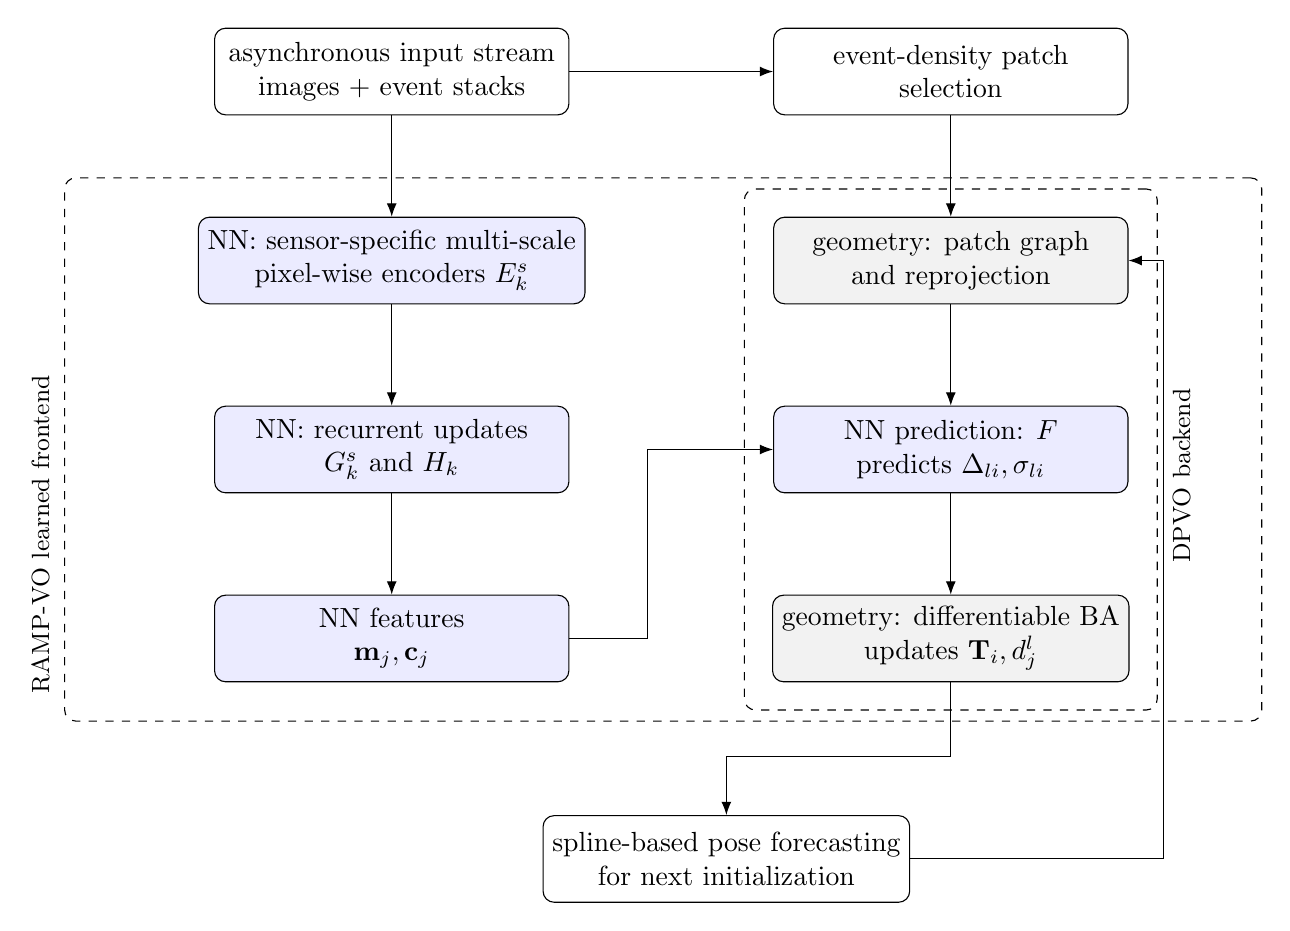
\begin{tikzpicture}[x=1cm,y=1cm,>=Latex]
  \tikzstyle{block}=[draw,rounded corners,minimum width=45mm,minimum height=11mm,align=center]
  \tikzstyle{nnblock}=[draw,rounded corners,fill=blue!8,minimum width=45mm,minimum height=11mm,align=center]
  \tikzstyle{geomblock}=[draw,rounded corners,fill=gray!10,minimum width=45mm,minimum height=11mm,align=center]

  \node[block] (stream) at (0,0) {asynchronous input stream\\images + event stacks};
  \node[nnblock] (pwe) at (0,-2.4) {NN: sensor-specific multi-scale\\pixel-wise encoders $E_k^s$};
  \node[nnblock] (recur) at (0,-4.8) {NN: recurrent updates\\$G_k^s$ and $H_k$};
  \node[nnblock] (feat) at (0,-7.2) {NN features\\$\mathbf{m}_j,\mathbf{c}_j$};

  \node[block] (patch) at (7.1,0) {event-density patch\\selection};
  \node[geomblock] (graph) at (7.1,-2.4) {geometry: patch graph\\and reprojection};
  \node[nnblock] (update) at (7.1,-4.8) {NN prediction: $F$\\predicts $\Delta_{li},\sigma_{li}$};
  \node[geomblock] (ba) at (7.1,-7.2) {geometry: differentiable BA\\updates $\mathbf{T}_i,d_j^l$};
  \node[block] (forecast) at (4.25,-10.0) {spline-based pose forecasting\\for next initialization};
  \coordinate (frontendleftpad) at ($(pwe.west)+(-1.2,0)$);
  \coordinate (frontendrightpad) at ($(update.east)+(1.2,0)$);
  \node[draw,dashed,rounded corners,fit=(pwe)(recur)(feat)(update)(frontendleftpad)(frontendrightpad),inner sep=14pt] (frontendbox) {};
  \node[draw,dashed,rounded corners,fit=(graph)(ba),inner sep=10pt] (backendbox) {};
  \node[fill=white,inner sep=1.5pt,anchor=east,rotate=90] at ($(frontendbox.west)+(-0.3,+1)$) {\small RAMP-VO learned frontend};
  \node[fill=white,inner sep=1.5pt,anchor=west,rotate=90] at ($(backendbox.east)+(0.3,-1.5)$) {\small DPVO backend};

  \draw[->] (stream) -- (pwe);
  \draw[->] (pwe) -- (recur);
  \draw[->] (recur) -- (feat);

  \draw[->] (patch) -- (graph);
  \draw[->] (graph) -- (update);
  \draw[->] (update) -- (ba);
  \coordinate (barouteA) at (7.1,-8.7);
  \coordinate (barouteB) at (4.25,-8.7);

  \draw[->] (ba.south) -- (barouteA) -- (barouteB) -- (forecast.north);

  \coordinate (toproute) at (4.25,0);
  \draw[->] (stream.east) -- (toproute) -- (patch.west);

  \coordinate (midroute) at (3.25,-7.2);
  \draw[->] (feat.east) -- (midroute) |- (update.west);

  \coordinate (feedbackrouteA) at (9.8,-10.0);
  \coordinate (feedbackrouteB) at (9.8,-2.4);
  \draw[->] (forecast.east) -- (feedbackrouteA) -- (feedbackrouteB) -- (graph.east);
\end{tikzpicture}
\caption{Block decomposition of RAMP-VO. The dashed left group is the RAMP-VO learned frontend, which processes asynchronous images and event stacks and predicts the features \(\mathbf{m}_j,\mathbf{c}_j\) together with the per-edge quantities \(\Delta_{li},\sigma_{li}\). The dashed right group is the DPVO backend inherited from DPVO, which builds reprojection constraints and runs bundle adjustment to update poses and depths.}
\end{figure}

\section{Main takeaways}

\begin{itemize}
    \item RAMP-VO inherits the DPVO philosophy: optimize poses and patch depths with differentiable bundle adjustment.
    \item The main novelty is the asynchronous recurrent encoder that fuses event stacks and images into a shared latent state.
    \item The network predicts patch-level corrections and confidences, not the full pose directly.
    \item Pose forecasting uses spline extrapolation of recent patch tracks to initialize future poses better.
    \item Events help not only because they add another modality, but because the latent state can be updated between image arrivals.
\end{itemize}

\appendix

\section{Appendix: technical details}

\subsection{LSTM Refresher}

An LSTM (Long Short-Term Memory) is a recurrent neural-network unit that updates an internal memory state and a hidden state over time. Given an input \(\mathbf{u}_t\), previous hidden state \(\mathbf{h}_{t-1}\), and previous cell state \(\mathbf{c}_{t-1}\), an LSTM computes gates that decide what information to forget, what new information to write, and what part of the internal memory to expose:
\begin{align}
\mathbf{f}_t &= \sigma(\mathbf{W}_f[\mathbf{u}_t,\mathbf{h}_{t-1}] + \mathbf{b}_f), \\
\mathbf{i}_t &= \sigma(\mathbf{W}_i[\mathbf{u}_t,\mathbf{h}_{t-1}] + \mathbf{b}_i), \\
\tilde{\mathbf{c}}_t &= \tanh(\mathbf{W}_c[\mathbf{u}_t,\mathbf{h}_{t-1}] + \mathbf{b}_c), \\
\mathbf{o}_t &= \sigma(\mathbf{W}_o[\mathbf{u}_t,\mathbf{h}_{t-1}] + \mathbf{b}_o), \\
\mathbf{c}_t &= \mathbf{f}_t \odot \mathbf{c}_{t-1} + \mathbf{i}_t \odot \tilde{\mathbf{c}}_t, \\
\mathbf{h}_t &= \mathbf{o}_t \odot \tanh(\mathbf{c}_t).
\end{align}
In RAMP-VO, the paper uses pixel-wise LSTMs, meaning that this recurrent update is applied independently at each pixel location of the feature maps. The role of the LSTM here is to give each sensor stream a temporal memory before the event/image information is fused into the shared state.

\subsection{Encoder Refresher}

In general, an encoder is a neural module that maps raw inputs into a feature representation that is more useful for the downstream task. In this paper, the raw inputs are images or event stacks, and the encoder produces feature maps that retain motion-relevant information while being easier for the tracking and optimization backend to use. The RAMP encoder is not a single block but a composition of three operations: sensor-specific feature extraction \(E_k^s\), temporal memory update \(G_k^s\), and asynchronous cross-sensor fusion \(H_k\). The output of this encoder is then turned into the matching and context features \(\mathbf{m}_j,\mathbf{c}_j\) consumed by the DPVO backend.

\subsection{Differentiable Bundle-Adjustment Layer}

In this paper, a \emph{differentiable bundle-adjustment layer} is a module that takes the current pose/depth variables, forms the reprojection residuals from Equation~\eqref{eq:main_ba}, and performs a fixed small number of optimization steps to reduce that objective. It is called a \emph{layer} because it is embedded inside the neural network pipeline, and it is called \emph{differentiable} because, during training, gradients are propagated not only through the feature-extraction and update blocks, but also through the optimizer steps themselves. In other words, the loss depends on the optimized variables after BA, and backpropagation differentiates through the computations that produced those optimized variables.

\subsection{Damped Nonlinear Least-Squares Updates}

The BA objective is nonlinear in the poses and depths, so it is minimized iteratively. Let the stacked residual vector be denoted by
\begin{equation}
\mathbf{r}(\mathbf{X}),
\end{equation}
with Jacobian
\begin{equation}
\mathbf{J} = \frac{\partial \mathbf{r}}{\partial \mathbf{X}}.
\end{equation}
At iteration \(k\), one linearizes the residual around the current estimate \(\mathbf{X}^{(k)}\), solves for an increment \(\delta \mathbf{X}\), and updates the state by
\begin{equation}
\mathbf{X}^{(k+1)} = \mathbf{X}^{(k)} + \delta \mathbf{X}.
\end{equation}
This additive notation is only a shorthand. In practice, the state contains both Euclidean variables and pose variables on \(\mathrm{SE}(3)\). If we write
\begin{equation}
\mathbf{X} = \left\{\mathbf{T}_i, d_j^l\right\},
\qquad
\delta \mathbf{X} = \left\{\delta \boldsymbol{\xi}_i, \delta d_j^l\right\},
\end{equation}
then the effective updates are
\begin{align}
\mathbf{T}_i^{(k+1)} &= \mathrm{Exp}(\delta \boldsymbol{\xi}_i)\,\mathbf{T}_i^{(k)}, \\
d_j^{l\,(k+1)} &= d_j^{l\,(k)} + \delta d_j^l.
\end{align}
In a Levenberg--Marquardt-style step, the increment is obtained from the damped normal equations
\begin{equation}
\left(\mathbf{J}\T \mathbf{W}\mathbf{J} + \lambda \mathbf{I}\right)\delta \mathbf{X}
= -\mathbf{J}\T \mathbf{W}\mathbf{r},
\end{equation}
that is,
\begin{equation}
\delta \mathbf{X}
= -\left(\mathbf{J}\T \mathbf{W}\mathbf{J} + \lambda \mathbf{I}\right)^{-1}\mathbf{J}\T \mathbf{W}\mathbf{r}.
\end{equation}
In the present note, \(\mathbf{W}\) can be written explicitly as
\begin{equation}
\mathbf{W} = \mathrm{blkdiag}\!\left(\{\sigma_{li}\}_{(l,i)\in\mathcal{E}}\right),
\end{equation}
that is, a block-diagonal matrix whose \(2\times 2\) blocks are the per-edge confidence matrices \(\sigma_{li}\) from Equation~\eqref{eq:main_ba}. These \(\sigma_{li}\) are predicted by the 
neural update operator \(F\), together with the corrections \(\Delta_{li}\); this learned weighting mechanism is part of the DPVO backend inherited by RAMP-VO. These are called \emph{residual weights} because they determine 
how strongly each residual contributes to the normal equations: a larger weight means that the corresponding 
reprojection error has a stronger influence on the update, while a smaller weight downweights that measurement. The scalar \(\lambda>0\) is a damping parameter. When \(\lambda\) is small, the step behaves 
like Gauss--Newton; when \(\lambda\) is larger, the step becomes more conservative and numerically stable. This is what is meant by ``damped nonlinear least-squares updates, in the spirit of Levenberg--Marquardt.''
 In the paper's DPVO backend, only a small fixed number of such updates is run inside the layer.

\subsection{Training of the Neural Components}

RAMP-VO is trained \emph{end-to-end}: the network runs the full pipeline, produces intermediate trajectory estimates, the loss is computed from these outputs, and gradients are backpropagated through the differentiable modules with the standard training step
\begin{equation}
\texttt{traj = net(\ldots)}, \qquad \texttt{loss = compute\_losses(traj,\ldots)}, \qquad \texttt{loss.backward()}.
\end{equation}
In this sense, the supervision is applied at the output of the whole system, not by assigning a separate local loss to each block. The trainable neural modules are the RAMP encoder blocks \(E_k^s,G_k^s,H_k\), the multi-scale fusion modules producing \(\mathbf{m}_j,\mathbf{c}_j\), and the DPVO backend modules that predict \(\Delta_{li}\) and \(\sigma_{li}\). The differentiable BA layer is part of the gradient path, so these losses propagate through the optimizer updates as well.

The practical training setup described by the paper is the following: RAMP-VO is trained on an event-augmented version of TartanAir, following the DPVO training scheme and hyperparameters, for \(350{,}000\) steps on sequences of \(15\) images and \(30\) event stacks. In the released implementation, the iterative refinement loop also contains explicit \texttt{detach()} operations on some state variables, so the training graph is end-to-end but kept computationally manageable rather than left to grow without bound across all refinement iterations.

\paragraph{Very simple training-step pseudo-algorithm.}
\begin{algorithm}[h]
\caption{One RAMP-VO Training Step}
\begin{algorithmic}[1]
\State sample one training sequence of images, event stacks, and ground-truth poses
\State run the full RAMP-VO forward pass with several internal refinement iterations
\State obtain the predicted trajectory / patch outputs
\State compute the training loss from these outputs
\State call \texttt{loss.backward()} to compute gradients
\State update the network weights with the optimizer
\end{algorithmic}
\end{algorithm}

\subsection{Training Losses}

The paper states that RAMP-VO is trained end-to-end, but it does not spell out the loss in the main text. The official training code defines the loss as a weighted sum of a patch-reprojection term and a relative-pose term, accumulated over the intermediate trajectory estimates returned by the network.

For one optimization stage and one active edge \((l,i)\), the code compares the predicted reprojected patch coordinates
\begin{equation}
\mathbf{P}_{ji}^{\prime l,\mathrm{pred}} = \omega(\mathbf{T}_i,\mathbf{T}_j,\mathbf{P}_j^l)
\end{equation}
with the corresponding ground-truth reprojected patch coordinates
\begin{equation}
\mathbf{P}_{ji}^{\prime l,\mathrm{gt}} = \omega(\mathbf{T}_i^{\mathrm{gt}},\mathbf{T}_j^{\mathrm{gt}},\mathbf{P}_j^{l,\mathrm{gt}}).
\end{equation}
In the released code these are the quantities called \texttt{coords} and \texttt{coords\_gt}. Let \(v_{li}\) be the corresponding validity mask. The code first forms the per-pixel patch error
\begin{equation}
e_{\mathrm{pix}} = \norm{\mathbf{P}_{ji}^{\prime l,\mathrm{pred}}-\mathbf{P}_{ji}^{\prime l,\mathrm{gt}}}_2,
\end{equation}
then reshapes each \(p\times p\) patch into \(p^2\) candidate pixel errors and keeps the minimum valid one. Denoting the resulting per-patch error by \(e\), the flow term is
\begin{equation}
\mathcal{L}_{\mathrm{flow}} = w_{\mathrm{flow}}\,\mathrm{mean}(e),
\end{equation}
where \(w_{\mathrm{flow}}\) is the training hyperparameter called \texttt{flow\_weight} in the code.

The pose term is built from relative poses. Using the same notation as in the rest of the document, let \(\mathbf{T}_i\) denote the predicted camera poses and \(\mathbf{T}_i^{\mathrm{gt}}\) the ground-truth poses. The code forms all pairwise relative motions
\begin{equation}
\Delta \mathbf{T}_{ij}^{\mathrm{pred}} = \mathbf{T}_i^{-1}\mathbf{T}_j,
\qquad
\Delta \mathbf{T}_{ij}^{\mathrm{gt}} = (\mathbf{T}_i^{\mathrm{gt}})^{-1}\mathbf{T}_j^{\mathrm{gt}},
\end{equation}
then measures the relative-pose error in the Lie algebra:
\begin{equation}
\mathbf{e}_{ij}^{\mathrm{pose}} = \mathrm{Log}\!\left(\Delta \mathbf{T}_{ij}^{\mathrm{pred}}(\Delta \mathbf{T}_{ij}^{\mathrm{gt}})^{-1}\right).
\end{equation}
This error is split into translation and rotation parts,
\begin{equation}
t_{ij} = \norm{\mathbf{e}_{ij,1:3}^{\mathrm{pose}}}_2,
\qquad
r_{ij} = \norm{\mathbf{e}_{ij,4:6}^{\mathrm{pose}}}_2,
\end{equation}
and the pose term is
\begin{equation}
\mathcal{L}_{\mathrm{pose}} = w_{\mathrm{pose}}\left(\mathrm{mean}(t_{ij}) + \mathrm{mean}(r_{ij})\right),
\end{equation}
where \(w_{\mathrm{pose}}\) is the hyperparameter called \texttt{pose\_weight}.

The total training loss used in the code is therefore
\begin{equation}
\mathcal{L} = \sum_{k}\left(\mathcal{L}_{\mathrm{flow}}^{(k)} + \mathcal{L}_{\mathrm{pose}}^{(k)}\right),
\end{equation}
with the dependency structure
\begin{equation}
\mathcal{L}_{\mathrm{flow}} = \mathcal{L}_{\mathrm{flow}}\!\left(\{\Delta_{li}\}_{(l,i)\in\mathcal{E}}\right),
\qquad
\mathcal{L}_{\mathrm{pose}} = \mathcal{L}_{\mathrm{pose}}\!\left(\{\mathbf{T}_i\},\{\Delta_{li},\sigma_{li}\}_{(l,i)\in\mathcal{E}}\right),
\end{equation}
where
\begin{equation}
(\Delta_{li},\sigma_{li}) = F(\mathbf{P}_{ji}^{\prime l},\mathbf{c}_i,\mathbf{m}_i,\mathbf{m}_j),
\qquad
(\mathbf{m}_j,\mathbf{c}_j)=K(\{\state_j^s\}_{s=0}^2).
\end{equation}
where \(k\) indexes the successive intermediate trajectory estimates produced during the iterative refinement.
\begin{itemize}
    \item \(\mathcal{L}_{\mathrm{flow}}\): supervises local patch correspondences; it directly constrains \(\Delta_{li}\) and indirectly constrains \(\mathbf{m}_j,\mathbf{c}_j\).
    \item \(\mathcal{L}_{\mathrm{pose}}\): supervises the global camera trajectory after bundle adjustment.
\end{itemize}
Only pose loss would give weak and indirect supervision to local patch matching, while only flow loss could give good local matches without the best global motion. In the released training code, the initial ``structure-only'' phase uses only \(\mathcal{L}_{\mathrm{flow}}\) for the first \(1000\) training steps.
This description comes from the released training code, not from an explicit formula in the paper.

\section{Appendix: performance discussion}

\subsection{Computational Performance Discussion}

The paper argues that RAMP-VO is designed to be computationally efficient at the encoder level because the RAMP encoder is highly parallelizable and avoids the more expensive sequential ConvGRU-style processing used by RAM-Net-like architectures. The strongest explicit evidence given in the paper is the timing comparison for feature extraction: on a Quadro RTX 8000 GPU, RAM Net takes \(370\) ms on average to extract features from a single frame or event stack, while the proposed RAMP encoder takes \(47\) ms, which the authors report as an \(8\times\) speedup.

At the same time, the overall method is not obviously cheap in an absolute sense. The system still combines multi-scale recurrent states, asynchronous event/image processing, learned patch refinement, and a differentiable bundle-adjustment backend. Moreover, the paper reports a substantial training cost: \(350{,}000\) training steps on sequences of \(15\) images and \(30\) event stacks, with roughly \(8\) days of training on a Quadro RTX 8000 GPU.

What the paper does \emph{not} provide is a detailed audit of full-system computational cost or memory usage. In particular, it does not report GPU memory consumption, parameter counts, FLOP counts, or a full end-to-end runtime breakdown separating the encoder, the update operator, and the BA backend.

The safest conclusion is the following: the paper explicitly shows that the RAMP encoder is much faster than a RAM-Net-like alternative, but neither the paper nor the released code provides a complete end-to-end compute or memory audit.

\subsection{Memory Usage Estimate}

Using the official implementation, one can estimate the persistent inference-time GPU buffers. With the default values \(N=2048\) buffered frames, \(M=80\) patches per frame, memory length \(\texttt{mem}=32\), resolution \(640\times 480\), patch size \(P=3\), and mixed precision enabled for the cached feature tensors, the persistent GPU buffers account for roughly
\begin{equation}
187 \text{ MiB}.
\end{equation}
The dominant term is the cached full-resolution feature tensor \(\texttt{fmap1\_}\), which alone occupies about \(150\) MiB.

To account for model parameters, one can use the released checkpoint sizes as a practical proxy. The official multi-scale checkpoint is \(88{,}269{,}981\) bytes, i.e.
\begin{equation}
84.2 \text{ MiB},
\end{equation}
while the official single-scale checkpoint is \(41{,}239{,}053\) bytes, i.e.
\begin{equation}
39.3 \text{ MiB}.
\end{equation}
Adding these to the persistent buffer estimate gives the following lower-bound inference-time memory estimates:
\begin{align}
\text{RAMP-VO multi-scale} &\approx 187 + 84.2 = 271.6 \text{ MiB}, \\
\text{RAMP-VO single-scale} &\approx 187 + 39.3 = 226.8 \text{ MiB}.
\end{align}
These numbers are only estimates and should be read as lower bounds. They do not include temporary activations inside the encoder and update operator, correlation volumes, BA workspaces, CUDA runtime overhead, or any training-time storage for gradients and optimizer states. Therefore the actual memory needed to run the full system is higher than these values, potentially by a substantial margin.

\end{document}
